\startchapter{AI-driven Software Engineering}
\label{chapter:Exp}

The current approaches focus on programming-in-the-small i.e, on individual lines of code. 
Code language models have focused (effectively!) on source code as language, implying the task is to predict the next token or series of tokens.
Thus support is for software \textit{coding} rather than software \emph{engineering}. 
What might AI support for software engineering require? 

There are areas of code suggestions that are not easily fixable or at least, not detectable efficiently before training or recommendation is required, at the time-scale of code completion (less than one second) \cite{}.
These problems align with a software abstraction hierarchy that sees code compilation and syntax checking at the least abstract level, and software architecture analysis and design at the most abstract level.
Figure \ref{fig:levels} exemplifies this. \neil{adapt for this paper - add AI, add line of tradeoff}
As we descend the levels, we have software concepts that are more difficult to automate (design rules vs code smells), that are nonetheless more important for software quality attributes (QA). 
We suggest that similarly, AI will struggle to offer useful suggestions lower down the list. 
The question remains where we stand today, and where the line (or area) exists between places where the AI should drive, and where a human engineer should take control.

\begin{figure}
    \centering
    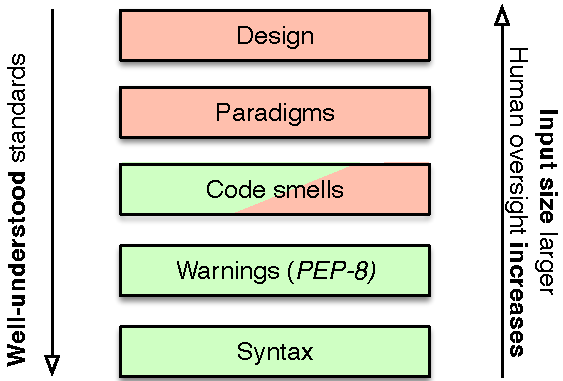
\includegraphics[width=.5\linewidth]{Figures/taxonomy-copilot.pdf}
    \caption{Hierarchy of software abstractions. Syntax reflects syntactically correct code and is warned by the compiler. Warnings include `-w' style compiler flags. Smells are aspects of source code that are sub-optimal by general acceptance; paradigms are idioms and good practices for languages and problems areas such as mobile computing. Finally, design refers to optimal design approaches for system qualities.}
    \label{fig:levels}
\end{figure}

We consider three scenarios. 
One is the way Copilot and AI-driven development manage language idioms.
A second is the way best practices are dealt with.
% \neil{third? maybe SQ smells design smells.}.

\section{Language idioms and paradigms}
We leveraged the work of Alexandru et.al\cite{Alexandru2018}, which identified common Python programming idioms, and compared how top 5 idioms from that work were suggested by Copilot.
We considered it a match if Copilot suggested the idiom in the first 2 suggestions, but note if the idiom appeared any of the top 10 suggestions currently viewable in Copilot. 

Copilot failed to suggest the recommended way for all the 5 idioms we tested, i.e, copilot did not have the recommended solution in its top 2 suggestions. However, 3 out of 5 idioms had the recommended way in its top 10 suggestions. The ranking metric for different suggestions made by copilot is currently unknown. So, we could not find the reason why Copilot is ranking a bad way over the good recommended way.

Below is the example of list comprehension idiom, showing the input, the top suggestion by Copilot and the recommended way suggested by Alexandru et.al \cite{Alexandru2018}.

\begin{tcolorbox}[title=List Comprehension,boxsep=.5mm]
    %https://tex.stackexchange.com/questions/337909/tcolorbox-tcbline-style
\textbf{Model Input:}
\begin{lstlisting}[language=Python]
#list comprehension

result_list = 
\end{lstlisting}
\tcbline
\textbf{Model Output:}
\begin{lstlisting}[language=Python]
result_list = []
for i in range(1,11):
    result_list.append(i)
\end{lstlisting}
\tcbline
\textbf{Recommended way:}
\begin{lstlisting}[language=Python]
result_list = [el for el in range(11)]
\end{lstlisting}
\end{tcolorbox}

\section{Best Practices}
We considered best practices for JavaScript development. 
To ground our practices we relied on the AirBNB JavaScript coding style guide \cite{airbnb_code}, a widely used coding style standard. 
There are a variety of best practices. 
We therefore chose practices that were closer to the the design level of the taxonomy, rather than the code level (e.g., trailing comma use).

For example, in JavaScript, callback api was used in the past to achieve concurrency which were replaced by promises. We checked if copilot suggests code which is specifically mentioned in the JavaScript documentation as a bad practice or an anti-pattern. Bad Practices in using promises for asynchronous JavaScript like not returning promises after creation, forgetting to terminate chains without catch statement, which are explained in documentation\footnote{\url{https://developer.mozilla.org/en-US/docs/Web/JavaScript/Guide/Using_promises}} and StackOverflow\footnote{\url{https://stackoverflow.com/questions/30362733/handling-errors-in-promise-all/}} are not known to copilot and suggested code with those common anti-patterns as they occur more frequently in copilot training data.

We chose 5 JavaScript coding standards from AirBNB JavaScript coding style guide \cite{airbnb_code}. We considered it a match if Copilot suggested the recommended way in the first 2 suggestions, but note if the recommended way appeared any of the top 10 suggestions. 

Copilot failed to suggest the recommended way for all the 5 standards we tested, i.e, copilot did not have the recommended way in its top 2 suggestions. only 1 out of 5 standards had the recommended way in its top 10 suggestions. 

Below is an example of logging a function , showing the input, the top suggestion by Copilot and the recommended way suggested by AirBNB coding style guide \cite{airbnb_code}.

\begin{tcolorbox}[title=Logging a Function,boxsep=.5mm]
    %https://tex.stackexchange.com/questions/337909/tcolorbox-tcbline-style
\textbf{Model Input:}
\begin{lstlisting}[language=JavaScript]
// logging function

class foo {
    bar ()
\end{lstlisting}
\tcbline
\textbf{Model Output:}
\begin{lstlisting}[language=JavaScript]
{
    console.log('bar');
    }
}
\end{lstlisting}
\tcbline
\textbf{Recommended way:}
\begin{lstlisting}[language=JavaScript]
class foo {
    bar (){ 
    console.log(this.bar) ;
}}
\end{lstlisting}
\end{tcolorbox}